\documentclass[a4paper,12pt]{article}
\usepackage[latin1]{inputenc}
\usepackage[spanish]{babel}
\usepackage{bm}
\usepackage{graphicx}
\usepackage{amsmath}
\usepackage{enumerate}
%\documentstyle[12pt,bezier]{articulo}
\setlength{\textheight}{235mm}
\setlength{\textwidth}{168mm}
\setlength{\oddsidemargin}{0pt}
\pagestyle{empty}

\begin{document}
\mbox{}\vspace*{-45mm}

{\centering
{\small\sc Escuela T�cnica Superior de Ingenieros de Caminos, Canales y
Puertos (Madrid)}\\*[4mm]
{\Large\bf M�todo de los Elementos Finitos}\\*[4mm]
PR�CTICA 3: Flujo en medios porosos \\*[4mm]
}
%%%%%
\noindent
La figura adjunta representa una pantalla pr�cticamente impermeable, hincada
sobre un terreno cuya permeabilidad es $k=8.47\cdot 10^{-5}$ m/s.
Para el nivel de agua indicado en dicha figura se desean analizar las
filtraciones. Se obtendr� la distribuci�n
de presiones (altura piezom�trica) y la distribuci�n de velocidades
horizontales y verticales. Asimismo se estimar� el caudal que es necesario
bombear con el fin de que el pozo permanezca seco.

\begin{center}
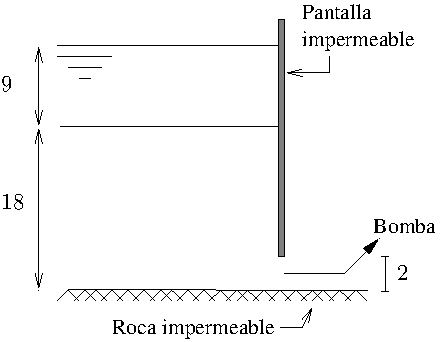
\includegraphics{practi3}
\end{center}
\end{document}
